\chapter{Initial Project Plan}
\label{app:projectPlan}
\section{Background}
We’re three game programming students, and naturally we are going to make a game to end our degree as that is what this bachelor is about. We want to use this project to learn valuable skills preparing us for the future. The design of the game allows us to focus on the networking aspects of game development. Figuring out good practices for local responsiveness coupled with consistent networked behaviour and how to implement these is something we would like to learn. This is good knowledge to have in a world where multiplayer, and the ability to stay connected is very important, even in games.
The amount of abilities will challenge us when it comes to game design and balance between a large amount of components, and will push our knowledge in the design aspect of game development. 

\section{Technology}
We’ll use Unity as a game engine. Unity is an engine used by a lot by Norwegian developers, and an engine heavily used worldwide~\cite{unityUsageStatistics}. We already have some experience with Unity, so we want to expand our knowledge. 
Using a game engine is beneficial because it allows us to focus on making a game, rather than constructing the components we need to create a game. 

We will be using Toggl as our primary tool for time tracking. It’s easy to use and allows us to track time spent by the team and what we spent time on. Another benefit of using Toggl is that it can be integrated to Jira allowing us to display time data directly in Jira. 

We will use a combination of Jira, Confluence and Bitbucket for project management and issue tracking, documenting and source code respectively. These are to be part of the professional programming course, and we already have some experience using these tools. They’re all part of Atlassian software development tools, which makes them fairly easy to integrate with each other.

Our primary IDE will be Visual Studio 2015 as it provides us with integrated testing tools with Unity like breakpoints and step by step debugging.  

Group communication will be done through Discord as all the group members are familiar with it and uses it regularly.

\section{Project Goals}
The goals of this project is to have a balanced and entertaining game at the end of semester. In addition to being robust in the sense of proper handling of disconnects, packet delays and packet loss.  During this project we want to learn and improve our Unity knowledge. We want to learn more about networking in Unity, how we effectively handle client/server verification and how we provide a consistent and responsive user experience locally. We also want to improve our knowledge regarding Artificial Intelligence by implementing player-like bots (possibly self-learning) and a “replay highlight selection”-AI if there is enough time. 

One of the other things we want more experience with is asymmetric balancing on a larger scale. We will have to balance individual abilities as well as entire kits. This has to be balanced towards multiple players using different kits in combination with each other. We will have to make sure that overall docking kit balance is somewhat good to avoid scenarios where everyone just uses the same docking kit because it is superior in each and every case. In the Standard Game Mode docking kits will have different prices, and therefore their strength needs to correspond the price.

Although the visuals are not our priority we’ll use Unity shaders for different visual effects, for instance abilities. The fog of war will be solved using masking shaders. We want to learn how to make use of professional tools such as Jira and Confluence for project management. We want to improve our ability to estimate the time it takes to implement features and work with smart/semantic commits for issue management.  

\section{Scope}
\subsection*{Areas of Expertise}
This project will include many disciplines from game development and game programming. The main parts of this will be gameplay design and balancing abilities for docking kits, and then network these. We’ll also need to handle user input, and the responsiveness challenge when it comes to users triggering networked abilities. We’ll have a user interface to display each ability and player health. Graphics and animations will be simplistic and somewhat abstract since this isn’t a priority, and we’re no artists.

\subsection*{Scope Limitations}
We will be focusing on finishing the standard game mode first and add a few docking kits. The scope is variable due to the nature of the game. It focuses on having a variety of abilities, and we can simply add/drop making more as the project goes on. The same goes for game modes.

\subsection*{Task Description}
Dockit League is a top-down multiplayer battle arena game in which players control vehicles that gets different abilities by equipping docking kits. 
Taking inspiration from key features in other popular games, we hope to make a fun and unique experience.

The Standard Game Mode features two teams that play against each other in multiple short rounds, before swapping sides. The sides are asymmetric, meaning if the round timer runs out, the attacking team loses. There will be control points around the map, the attacking team needs to conquer one of these in order to win the round.

Each player can equip one docking kit. These kits consist of four abilities each. In the Standard Game Mode these kits may be bought during the buy time at round start, and the price will vary depending on kit strength. This means that a player will have to save their currency over multiple rounds in order to get any kit.
Most of the abilities have some sort of interaction between each other, both within a docking kit, and with other kits. This allows teams to choose between different strategies, either for executing a strategy themselves, or to counter the enemy's strategy.

The players will have a field of view and a sight radius, the size of these may vary depending on their equipped docking kits. Areas outside of this field will be fog of war. 

\section{Project Structure}
\subsection*{Roles, Responsibilities}
We have divided the group into roles and responsibilities. Martin has been appointed as project lead while Andreas and Sondre are developers. Other responsibilities:
\begin{description}
    \item[Andreas:] Documenting meetings/decisions
    \item[Martin:] Scrum Master
\end{description}

\subsection*{Group rules and routines}
We have outlined some group rules as an attachment to the project agreement. Other than those, some general routines will be to document all design decisions and write short summaries from all meetings in Confluence. All group members are required to show up to meetings. If this is not possible, a notification from the missing group member is needed beforehand.

\section{Planning, supervision and documentation}
\subsection*{Choice of system engineering model}
We have decided to use Scrum for this project. Developing games is generally an agile and iterative process, and being flexible is a must. Therefore an agile model like Scrum is ideal for the project.  Another reason for Scrum is that we wish to learn using professional tools like Jira and Confluence. Scrum works nicely with both of these. Finally, using Scrum allows us to generate a lot of extra documentation during the project due to the amount of meetings, which is going to be quite useful when writing the thesis itself. 

We are planning to have fortnightly sprints with daily standup meetings. Thursdays will be used for “sprint meetings” consisting of the review, retrospective and planning meeting. Each meeting will have a short summary written which will be added to the Confluence pages. 

\subsection*{Plan for status meetings and decision points}
We do not have any external clients for this project, but we will have regular status meetings with Simon McCallum who is the project supervisor. 

\section{Quality Assurance}
\subsection*{Documentation and code standard}
We will be using a good amount of Atlassian’s available tools for the project. Confluence will be used for documentation and as the thesis container while Jira will be used for management of Scrum and issues. 
We are going to enforce a common coding convention that all group members are required to use. The project’s coding convention is going to be the “One True Brace” style. We will also be using doxygen style comments for functions. 

\subsection*{Configuration management}
We will be using a Bitbucket repository with git as our primary means of version control and source code storage. The repository will be separated into several branches: 
\begin{itemize}
    \item We will have a master branch that always has a stable build of the project. This branch will generally get updated after sprints are done.
    \item There will be a development branch where we add features that are in development during sprints.
    \item Each member also has his own branch where work is done and merged into the development branch once the work is done. 
\end{itemize}

\subsection*{Testing and issue tracking}
Playtesting is something that we will do on a daily basis as we implement the various features we are working on. 
Issue tracking is going to be handled through Jira using smart commits when pushing code to the Bitbucket repository.

\section{Implementation plan}
\subsection*{Gantt chart}
\begin{figure}[thpb]
    \centering
    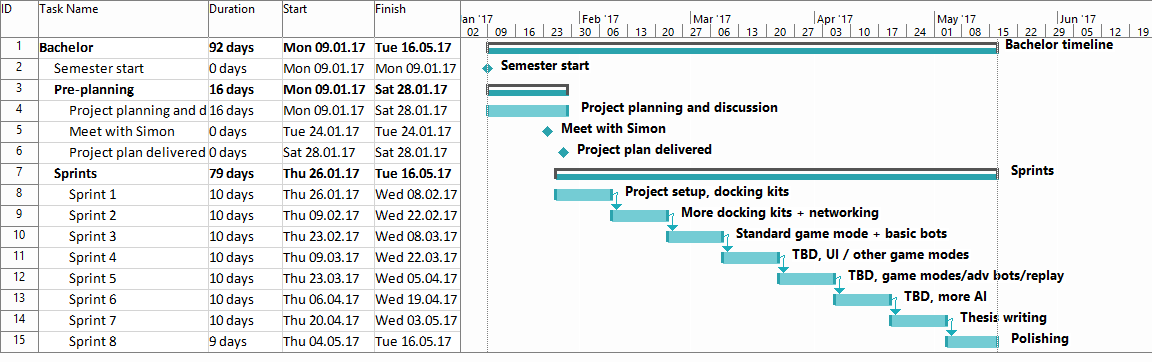
\includegraphics[width=1\textwidth]{images/gantt}
    \caption{Gantt chart from initial project plan}
    \label{fig:gantt}
\end{figure}

\subsection*{Milestones and Decisions}
We currently only have two major milestones in mind for the project. The first milestone is a working prototype of the game with a finished docking system. The second milestone is to have a working prototype with the standard game mode implemented. Due to the variable scope of the project it’s hard to estimate further milestones after this at this time.

All important design decisions and sprint meeting summaries will be documented in Confluence. The thesis itself will also be written directly in Confluence and later extracted to a PDF file. 

\subsection*{Time and resouce plan}
Time and resource planning will be done with the help of planning poker using story points, which will be done during the fortnightly sprint meetings, in accordance to our Scrum model. 